\documentclass{article}

% Language setting
% Replace `english' with e.g. `spanish' to change the document language
\usepackage[english]{babel}

% Set page size and margins
% Replace `letterpaper' with `a4paper' for UK/EU standard size
\usepackage[letterpaper,top=2cm,bottom=2cm,left=3cm,right=3cm,marginparwidth=1.75cm]{geometry}
\usepackage[section]{placeins}
% Useful packages
\usepackage{comment}
\usepackage{amsmath}
\usepackage{graphicx}
\usepackage[colorlinks=true, allcolors=blue]{hyperref}
\usepackage{PRIMEarxiv}
\usepackage[utf8]{inputenc} % allow utf-8 input
\usepackage[T1]{fontenc}    % use 8-bit T1 fonts
%\usepackage[hidelinks]{hyperref}       % hyperlinks
%\usepackage{url}            % simple URL typesetting
\usepackage{booktabs}       % professional-quality tables
\usepackage{amsfonts}       % blackboard math symbols
\usepackage{nicefrac}       % compact symbols for 1/2, etc.
\usepackage{microtype}      % microtypography
\usepackage{lipsum}
\usepackage{fancyhdr}       % header
\usepackage{graphicx}       % graphics
\graphicspath{{media/}}     % organize your images and other figures under media/ folder
\usepackage{array}
\usepackage{amsmath}
\usepackage{enumitem}
\newlist{rqs}{enumerate}{1}
\setlist[rqs]{label*=\textbf{RQ\arabic*}}
\newcommand\bulletparagraph[1]{\quad\textbullet\ \textbf{#1}}

% 3.1.1 hightligh
\usepackage{color}
\newcommand{\red}[1]{\textcolor{red}{#1}}
\newcommand{\authnote}[2]{{\bf[\textcolor{red}{#1}: \textcolor{blue}{#2}]}}
\newcommand{\an}[2]{{\bf[\textcolor{blue}{#1}: \textcolor{red}{#2}]}}
\newcommand{\greenote}[2]{{\bf[\textcolor[rgb]{0,0.5,0}{#1}: \textcolor[rgb]{0,0.5,0}{#2}]}}

\newcommand{\prog}{\ensuremath{{\cal P}}\xspace}
\newcommand{\true}{{\bf T}\xspace}
\newcommand{\false}{{\bf F}\xspace}
\newcommand{\Z}{\ensuremath{\mathbb{Z}}}
\newcommand{\xor}{\ensuremath{\oplus}}
\newcommand{\bool}{\texttt{Bool}}

\newcommand{\code}[1]{\texttt{#1}}

%\newcommand{\sysname}{{\sc Eponym}\xspace}
% \newcommand{\sysname}{{\sc BinSymn}\xspace}
\newcommand{\sysname}{{\scshape SymLM}\xspace}
% \newcommand{\sysnamebf}{{\sc\bf SymLM}\xspace}
% \newcommand{\sysnamebf}{{\scshape SymLM}\xspace}

\newcommand{\eg}{\textit{e.g.}\xspace}
\newcommand{\ie}{\textit{i.e.}\xspace}
\newcommand{\etc}{\textit{etc.}\xspace}
\newcommand{\etal}{\textit{et al.}\xspace}
\newcommand{\locationmanager}{\texttt{Lo\-ca\-tion\-Ma\-na\-ger}\xspace}
\newcommand{\locationprovider}{\texttt{Lo\-ca\-tion\-Pro\-vi\-der}\xspace}
\newcommand{\allowmocklocations}{\texttt{ALLOW\-\_MOCK\-\_LOCA\-TIONS}\xspace}
\newcommand{\isfrommockprovider}{\texttt{is\-From\-Mock\-Pro\-vi\-der()}\xspace}

% \renewcommand\footnotetextcopyrightpermission[1]{} % 

\newcommand{\myparagraph}[1]{\vspace{0.5em}\noindent{\bf #1}.}

\newcommand\featuretext[1]{%
  \llap{\vrule width.5pt height2pt depth2.5pt\kern2pt}%
  \rlap{\rotatebox{30}{\textbf{#1}}}%
}

\newcommand{\tick}{\ding{52}}
\newcommand{\tickNo}{\hspace{1pt}\ding{55}}

\newcommand{\Xin}[1]{{\authnote{Xin}{#1}}}

\newcommand{\ignore}[1]{}

\renewcommand{\paragraph}[1]{\vspace{0.12in}\noindent{\bf{#1}.}}

\newcommand{\sectionspace}{\vspace{0.00in}}
\newcommand{\subsectionspace}{\vspace{0.02in}}

\newcommand{\refspace}{\vspace{-0.08in}}

\newcommand{\erick}[1]{{\authnote{Erick}{#1}}}
\newcommand{\garrnote}[1]{{\greenote{Do This Garrett}{#1}}}

\newcommand*\circled[1]{\tikz[baseline=(char.base)]{
    \node[shape=circle,draw,inner sep=0.5pt] (char) {#1};}}
%Header
\pagestyle{fancy}
\thispagestyle{empty}
\rhead{ \textit{ }}

\title{Introduction to Algorithms - Solutions and Notes}
\author{Chufeng Jiang}

\begin{document}
\maketitle

Refer to the website to access its resources: \href{https://mitpress.mit.edu/9780262046305/introduction-to-algorithms/}{Introduction to Algorithms, fourth edition} \cite{10.5555/1614191}

\section{Chapter 1 The Role of Algorithms in Computing}\label{sec:Chapter 1 The Role of Algorithms in Computing}

\subsection{Exercises 1} 

\subsubsection{Describe your own real-world example that requires sorting. Describe one that requires finding the shortest distance between two points.}

A real-world example that requires sorting is the organization of books in a library. Libraries contain thousands of books that need to be effectively organized and managed so that patrons can easily find the book they're looking for. This often involves sorting books based on attributes such as title, author, subject, or ISBN. Through sorting, librarians can quickly locate a book's position, and readers can also find the specific location of the needed book via the catalog system.

An example that requires finding the shortest distance between two points is a GPS navigation system. When a user inputs a starting point and a destination, the GPS system calculates multiple possible routes and identifies the shortest or, considering traffic conditions, the quickest route. This involves solving the shortest path problem, a well-known problem in graph theory, typically using algorithms like Dijkstra's algorithm or the A* algorithm. This calculation takes into account not just the physical distance of roads but also factors such as traffic conditions and road restrictions to ensure that the user can reach their destination in the shortest or quickest possible time.

\subsubsection{Other than speed, what other measures of efficiency might you need to consider in a real-world setting?}

In real-world settings, several measures of efficiency beyond speed are crucial to consider, depending on the context and objectives. Here are a few significant ones:

\begin{enumerate}[leftmargin=2em]

\item[(1)] Cost Efficiency: Often, the cost is as important as speed. Whether it’s the cost of running a machine, the expense involved in transporting goods, or the cost of executing a digital operation, finding the most cost-effective solution is crucial for sustainability and profitability.

\item[(2)] Energy Efficiency: In many scenarios, especially those involving physical operations or manufacturing, energy consumption becomes a critical factor. Energy-efficient processes are not only better for the environment but can also reduce operational costs significantly.

\item[(3)] Resource Utilization: This refers to the optimal use of resources, including human resources, materials, and time. Efficient resource utilization ensures that you're getting the most out of the resources available to you without waste.

\item[(4)] Accuracy and Precision: In tasks that require a high degree of accuracy, such as data entry or medical diagnostics, the quality of the outcome is a vital measure of efficiency. Speed is irrelevant if the results are inaccurate or imprecise.

\item[(5)] Scalability: The ability to handle growing amounts of work, or its potential to be enlarged, is crucial in assessing the efficiency of processes, especially in fast-growing industries or businesses.

\item[(6)] Reliability: and Availability: The consistency of performance and the ability to be operational when needed are important. This is especially true for services and systems that require high uptime, such as IT services, manufacturing plants, and public utilities.

\item[(7)] Sustainability: The long-term viability of a process or product, with minimal negative impact on the environment or society, is increasingly being recognized as an essential aspect of efficiency.

\item[(8)] User Satisfaction: In service-oriented sectors, the efficiency of a process is also measured by the level of satisfaction it brings to its users or customers. Quick service might not be efficient if it doesn’t meet the users’ needs or expectations.

\item[(9)] Flexibility and Adaptability: The ability to adapt to changing circumstances or demands without significant drops in efficiency is crucial for long-term success in most fields.

\end{enumerate}

Considering these varied dimensions of efficiency can provide a more holistic view of what it means to be efficient in different contexts, often leading to better decision-making and outcomes.

\subsubsection{Select a data structure that you have seen previously, and discuss its strengths and limitations.}

One commonly used data structure is the Binary Search Tree (BST). A BST is a binary tree where each node has a key greater than all the keys in the node's left subtree and less than those in its right subtree. This property makes BSTs efficient for operations like search, insertion, and deletion.

\textbullet{ Strengths:}

\begin{enumerate}[leftmargin=2em]

\item[(1)] Ordered Structure: BSTs maintain their elements in a sorted order, which allows for efficient in-order traversal. This is particularly useful for tasks that require sorted data, such as printing all elements in a range.

\item[(2)] Dynamic: BSTs can grow or shrink as needed, allowing for dynamic data storage. They don't have a fixed size like arrays, making them more flexible for applications where the volume of data fluctuates.

\item[(3)] Efficient Operations: When balanced, the operations of search, insertion, and deletion can be performed in O(log n) time, where n is the number of nodes. This efficiency is due to the binary nature of BST, which cuts the search space in half with each comparison.

\item[(4)] Simplicity: BSTs are relatively simple to implement and understand, making them a popular choice for many applications.
\end{enumerate}

\textbullet{ Limitations:}

\begin{enumerate}[leftmargin=2em]
\item[(1)] Balancing: One of the significant limitations of BSTs is that they can become unbalanced with certain sequences of insertions and deletions, degrading performance to O(n) in the worst case. This happens when nodes are inserted in an already sorted manner, resulting in a tree that resembles a linked list.

\item[(2)] Space Overhead: Each node in a BST requires additional space for two pointers (left and right), which can be a significant overhead for trees with a large number of nodes, especially if the data stored in each node is small.

\item[(3)] Complex Balancing Algorithms: While there are self-balancing BSTs like AVL trees and Red-Black trees, implementing and maintaining these structures can be complex and error-prone.

\item[(4)] Not Cache-Friendly: BSTs do not ensure locality of reference. Traversing a BST can lead to frequent cache misses, especially in deep trees, since nodes are often not stored in contiguous memory locations.
\end{enumerate}
In summary, BSTs offer an efficient and flexible means of storing and retrieving ordered data when they are balanced. However, their performance can significantly degrade if they become unbalanced, and maintaining balance can introduce complexity. This trade-off between efficiency and complexity is a crucial consideration when choosing to use BSTs in applications.

\subsubsection{How are the shortest-path and traveling-salesman problems given above similar? How are they different?}

he Shortest Path Problem (SPP) and the Traveling Salesman Problem (TSP) are both fundamental problems in the field of graph theory, often applied in network analysis, logistics, and computer science. Despite their similarities, they address different challenges and have unique complexities.

\textbullet{ Similarities:}
\begin{enumerate}[leftmargin=2em]
\item[(1)] Graph-Based Problems: Both are solved within the framework of graph theory, where locations are represented by nodes and the paths between them by edges. The solutions involve traversing these edges to achieve a specific objective.

\item[(2)] Path Finding: Each problem involves finding a path that optimizes a certain criterion; in SPP, it's the minimum distance or cost between two points, while in TSP, it's the shortest possible route that visits each node exactly once and returns to the starting point.

\item[(3)] Optimization Problems: Both SPP and TSP are optimization problems. SPP seeks to minimize the path length (or cost) between two nodes, and TSP looks for the minimum cost circuit that visits all nodes.

\item[(4)] Use of Algorithms: Solutions to both problems often involve sophisticated algorithms. For example, Dijkstra's algorithm for SPP and various approximation, heuristic, or brute-force algorithms for TSP.

\end{enumerate}

\textbullet{ Differences:}

\begin{enumerate}[leftmargin=2em]

\item[(1)] Complexity and Solvability: SPP is typically a less complex problem with polynomial-time algorithms available for most of its variations (e.g., Dijkstra's algorithm for weighted graphs without negative cycles). TSP, on the other hand, is NP-hard, meaning that no polynomial-time solution exists for solving all instances of the problem, and heuristic or approximation methods are often used.

\item[(2)] Problem Scope: SPP focuses on finding the shortest path between two specific nodes in a graph. TSP, however, involves visiting all nodes in the graph exactly once and returning to the start, which adds a level of complexity not present in SPP.

\item[(3)] Applications: While both problems have wide-ranging applications, SPP is often used in routing and navigation systems, such as GPS technology, to find the shortest route between two locations. TSP is more commonly applied in logistics and planning, such as determining the most efficient route for delivery trucks that must visit multiple locations.

\item[(4)] Goal Specificity: The goal of SPP is very specific – find the shortest or least costly path between two points. In contrast, TSP seeks a global solution that takes into account all nodes in the network, requiring a comprehensive approach to problem-solving.

\end{enumerate}

In summary, SPP's more straightforward and efficient solutions contrast with TSP's complexity and the need for approximation or heuristic strategies to find near-optimal solutions.

\subsubsection{Come up with a real-world problem in which only the best solution will do. Then come up with one in which a solution that is "approximately" the best is good enough.}

\textbullet{ Real-World Problem Requiring the Best Solution:}

Aerospace Engineering - Spacecraft Trajectory Design: In the design of spacecraft trajectories, especially for missions that involve landing on other planets or moons, only the best solution will do. This involves calculating the precise path a spacecraft should take to reach its destination with minimal fuel consumption while avoiding obstacles like asteroids and accounting for gravitational forces from celestial bodies. The calculations must be exact to ensure the spacecraft enters the target planet's orbit or lands at a specific location at the right time. Any deviation from the optimal path could result in mission failure, loss of the spacecraft, or significant additional costs to correct the trajectory. This problem requires absolute precision because the safety of the mission and its crew (if manned), the integrity of the spacecraft, and the mission's scientific goals are all at stake.

\textbullet{ Real-World Problem Where an Approximate Solution Is Sufficient:}

Digital Marketing - Ad Placement Strategy: In digital marketing, particularly in the placement of ads on websites and social media, a solution that is "approximately" the best is often good enough. The objective is to maximize the return on investment (ROI) by targeting ads at the right audience, at the right time, and in the right place. However, given the complexities of human behavior, the changing dynamics of the internet, and the sheer volume of data, it's nearly impossible and not cost-effective to find the absolute best solution. Instead, marketers use algorithms and machine learning models to analyze trends and predict where ads are likely to be most effective. These models provide approximate solutions that, while not perfect, are effective enough to significantly increase visibility, engagement, and conversion rates. In this context, being approximately right can lead to a successful campaign that meets or exceeds its goals, even if it's not the absolute optimal solution in every scenario.


\subsubsection{Describe a real-world problem in which sometimes the entire input is available before you need to solve the problem, but other times the input is not entirely available in advance and arrives over time}

\subsubsection{ }

\subsubsection{ }

\subsubsection{ }

\subsubsection{ }





\subsection{How to add Figures}
\FloatBarrier
\begin{figure}[!ht]
\centering
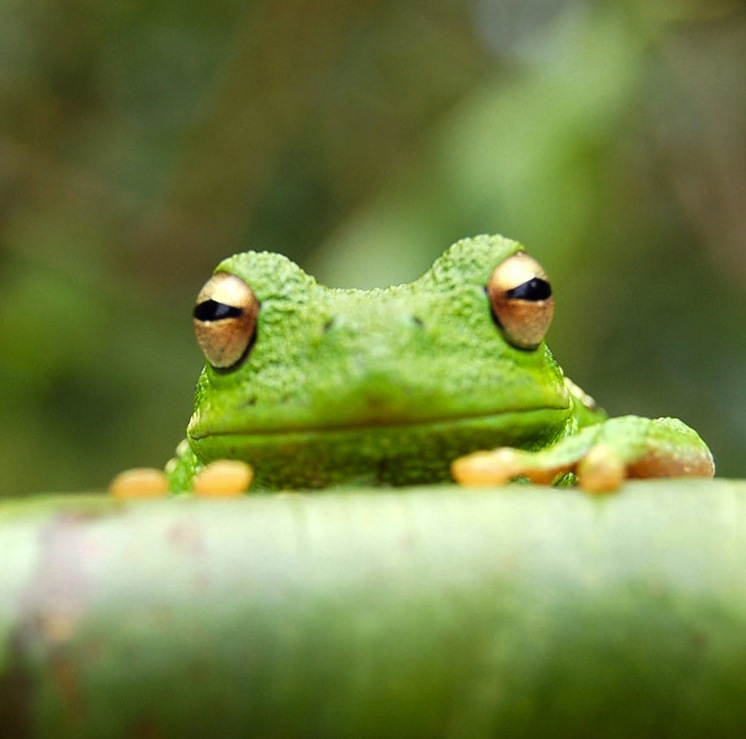
\includegraphics[width=0.25\linewidth]{./figures/frog.jpg}
\caption{\label{fig:frog}This frog was uploaded via the file-tree menu.}
\end{figure}
\FloatBarrier
\subsection{How to add Tables}

Use the table and tabular environments for basic tables --- see Table~\ref{tab:widgets}, for example. For more information, please see this help article on \href{https://www.overleaf.com/learn/latex/tables}{tables}. 
\FloatBarrier
\begin{table}[!ht]
\centering
\begin{tabular}{l|r}
Item & Quantity \\\hline
Widgets & 42 \\
Gadgets & 13
\end{tabular}
\caption{\label{tab:widgets}An example table.}
\end{table}
\FloatBarrier
\subsection{How to add Comments and Track Changes}

Comments can be added to your project by highlighting some text and clicking ``Add comment'' in the top right of the editor pane. To view existing comments, click on the Review menu in the toolbar above. To reply to a comment, click on the Reply button in the lower right corner of the comment. You can close the Review pane by clicking its name on the toolbar when you're done reviewing for the time being.

Track changes are available on all our \href{https://www.overleaf.com/user/subscription/plans}{premium plans}, and can be toggled on or off using the option at the top of the Review pane. Track changes allow you to keep track of every change made to the document, along with the person making the change. 

\subsection{How to add Lists}

You can make lists with automatic numbering \dots

\begin{enumerate}
\item Like this,
\item and like this.
\end{enumerate}
\dots or bullet points \dots
\begin{itemize}
\item Like this,
\item and like this.
\end{itemize}

\subsection{How to write Mathematics}

\LaTeX{} is great at typesetting mathematics. Let $X_1, X_2, \ldots, X_n$ be a sequence of independent and identically distributed random variables with $\text{E}[X_i] = \mu$ and $\text{Var}[X_i] = \sigma^2 < \infty$, and let
\[S_n = \frac{X_1 + X_2 + \cdots + X_n}{n}
      = \frac{1}{n}\sum_{i}^{n} X_i\]
denote their mean. Then as $n$ approaches infinity, the random variables $\sqrt{n}(S_n - \mu)$ converge in distribution to a normal $\mathcal{N}(0, \sigma^2)$.


\subsection{How to change the margins and paper size}

Usually the template you're using will have the page margins and paper size set correctly for that use-case. For example, if you're using a journal article template provided by the journal publisher, that template will be formatted according to their requirements. In these cases, it's best not to alter the margins directly.

If however you're using a more general template, such as this one, and would like to alter the margins, a common way to do so is via the geometry package. You can find the geometry package loaded in the preamble at the top of this example file, and if you'd like to learn more about how to adjust the settings, please visit this help article on \href{https://www.overleaf.com/learn/latex/page_size_and_margins}{page size and margins}.



\bibliographystyle{unsrt}
\bibliography{references}

\end{document}